\documentclass[11pt,a4paper]{ltjsarticle} % LuaLaTeX-ja用の日本語対応クラス(A4・11pt)
\usepackage{luatexja} % LuaLaTeXで日本語を扱うための基本パッケージ
\usepackage{luatexja-fontspec} % LuaLaTeXで日本語フォントを指定するための拡張
\usepackage{amsmath,amssymb} % 数式環境・記号の拡張
\usepackage{geometry} % 余白などページレイアウトの調整
\geometry{left=2.5cm,right=2.5cm,top=3cm,bottom=3cm} % ページ余白の具体的な設定
\usepackage{graphicx} % 画像の挿入
\usepackage{booktabs} % 表の罫線を美しくする
\usepackage{siunitx} % SI単位系の表記を統一・自動調整
\sisetup{detect-all,detect-weight=true,detect-family=true} % siunitxの細かい設定(フォント検出など)
\usepackage[
  unicode,bookmarks=true,bookmarksnumbered=true,hypertexnames=false,breaklinks=true,linktocpage=true,
  colorlinks=true,linkcolor=blue,citecolor=blue,urlcolor=blue,pdfborder={0 0 0},pdfpagelabels=false
]{hyperref} % PDFの目次やリンクを有効化・色付け
\usepackage{url} % URLを自動でリンク化
\usepackage{fancyhdr} % ヘッダー・フッターのカスタマイズ
\usepackage{fontspec} % 欧文フォントの指定(LuaLaTeX用)
\usepackage{unicode-math} % 数式フォントの指定(LuaLaTeX用)
\usepackage{pgfplots} % グラフ描画用パッケージ
\usepackage{tikz} % TikZ描画パッケージ
\pgfplotsset{compat=1.18} % バージョン互換性

% 欧文フォント設定(例: Times New Roman)
\setmainfont{Times New Roman} % 本文の欧文フォント
\setsansfont{Arial} % 欧文のサンセリフ体
\setmonofont{Consolas} % 欧文の等幅フォント

% 日本語フォント設定
\setmainjfont{Yu Mincho} % 本文の和文明朝体
\setsansjfont{Yu Gothic} % 和文ゴシック体

% 数式フォントもTimes系に統一
\setmathfont{XITS Math} % 数式用フォント(Times系互換)

\pagestyle{fancy} % ヘッダー・フッターのカスタムを有効化
\fancyhead{} % 既存のヘッダーをクリア
\fancyhead[R]{\footnotesize
  制御工学 周波数応答演習問題解答 \\
  長野高専 電気電子工学科 5年 34番 栁原魁人 \\
  2025年7月14日
} % 右上ヘッダーに情報を表示
% ヘッダー高さ警告の対策
\setlength{\headheight}{34.832pt} % ヘッダー高さを警告値に合わせて調整

\begin{document}

\section*{周波数応答演習問題 解答と解説}

周波数応答解析は、正弦波入力に対するシステムの定常応答(ゲインと位相)を周波数の関数として評価する手法です。伝達関数 $G(s)$ の複素変数 $s$ を $s=j\omega$ と置換することで周波数伝達関数 $G(j\omega)$ を得ます。ボード線図は、この $G(j\omega)$ のゲイン $|G(j\omega)|$ と位相 $\angle G(j\omega)$ を、それぞれ対数スケールの角周波数 $\omega$ に対してプロットしたもので、システムの周波数特性を直感的に理解するために不可欠です。

\section{問題5の解答}
\textbf{図6-16のボード線図で表される要素の伝達関数を求める。}

\subsection*{ステップ1:漸近線の特徴からシステムの構造を推定する}
与えられたゲイン線図の漸近線を観察します。
\begin{itemize}
    \item 低周波域 ($\omega < 20$ rad/s): 傾きが 0 dB/dec の水平な直線です。これはシステムのゲインが周波数に依存しないことを意味し、\textbf{比例要素 $K$} の存在を示唆します。
    \item 高周波域 ($\omega > 20$ rad/s): 傾きが -20 dB/dec の直線です。これはゲインが周波数の1乗に反比例して減少することを意味し、\textbf{1次遅れ要素 $\frac{1}{1+Ts}$} の存在を示唆します。
\end{itemize}
これらの観察から、システムの伝達関数は比例要素と1次遅れ要素の積で構成される、以下の形で表せると推定できます。
\begin{equation}
    G(s) = K \cdot \frac{1}{1+Ts} = \frac{K}{1+Ts}
\end{equation}

\subsection*{ステップ2:低周波域のゲインから比例定数 $K$ を求める}
低周波域の漸近線は、ゲインが一定値 23 dB を示しています。これは比例要素 $K$ のゲインに対応します。
\begin{align*}
    20 \log_{10}(K) &= 23 \\
    \log_{10}(K) &= \frac{23}{20} = 1.15 \\
    K &= 10^{1.15} \approx 14.1
\end{align*}

\subsection*{ステップ3:折点角周波数から時定数 $T$ を求める}
ゲイン線図の傾きが 0 dB/dec から -20 dB/dec に変化する点を\textbf{折点角周波数}と呼びます。グラフから、折点角周波数は $\omega_c = 20$ rad/s です。
1次遅れ要素の折点角周波数は、時定数 $T$ と $\omega_c = 1/T$ の関係にあります。
\begin{equation*}
    T = \frac{1}{\omega_c} = \frac{1}{20} = 0.05 \text{ s}
\end{equation*}

\subsection*{ステップ4:伝達関数を確定する}
ステップ2と3で求めた $K$ と $T$ の値を式(1)に代入し、伝達関数を確定します。
\begin{equation}
    G(s) = \frac{14.1}{1+0.05s}
\end{equation}

\section{問題6の解答}
\textbf{図6-17のボード線図で表される要素の伝達関数を求める。}

\subsection*{ステップ1:漸近線の特徴からシステムの構造を推定する}
ゲイン線図の漸近線の傾きの変化を観察します。
\begin{itemize}
    \item 低周波域 ($\omega < 0.1$): 傾きが \textbf{-20 dB/dec}。これは\textbf{積分要素 $\frac{1}{s}$} の存在を示します。
    \item 第1折点 ($\omega_{c1} = 0.1$): 傾きが -20 から -40 dB/dec に変化。傾きが-20だけ加算されており、これは\textbf{1次遅れ要素 $\frac{1}{1+T_1s}$} の存在を示します。
    \item 第2折点 ($\omega_{c2} = 2$): 傾きが -40 から -60 dB/dec に変化。同様に、これも\textbf{1次遅れ要素 $\frac{1}{1+T_2s}$} の存在を示します。
\end{itemize}
これらの要素と、全体的なゲインを調整する比例要素 $K$ を組み合わせることで、伝達関数は以下の形と推定できます。
\begin{equation}
    G(s) = K \cdot \frac{1}{s} \cdot \frac{1}{1+T_1s} \cdot \frac{1}{1+T_2s} = \frac{K}{s(1+T_1s)(1+T_2s)}
\end{equation}

\subsection*{ステップ2:折点角周波数から時定数 $T_1, T_2$ を求める}
各折点角周波数から、対応する1次遅れ要素の時定数を計算します。
\begin{align*}
    T_1 &= \frac{1}{\omega_{c1}} = \frac{1}{0.1} = 10 \text{ s} \\
    T_2 &= \frac{1}{\omega_{c2}} = \frac{1}{2} = 0.5 \text{ s}
\end{align*}

\subsection*{ステップ3:ゲイン定数 $K$ を求める}
ゲイン定数 $K$ は、低周波域の漸近線から求めます。この領域では、$s=j\omega$ が小さいため、$1+T_1s \approx 1$ および $1+T_2s \approx 1$ と近似できます。したがって、
\begin{equation*}
    G(j\omega) \approx \frac{K}{j\omega}
\end{equation*}
このゲインをdBで表すと、
\begin{equation*}
    |G(j\omega)|_{\text{dB}} = 20\log_{10}\left|\frac{K}{j\omega}\right| = 20\log_{10}\left(\frac{K}{\omega}\right) = 20\log_{10}(K) - 20\log_{10}(\omega)
\end{equation*}
グラフから、この直線は点 ($\omega$, \text{gain}) = (0.1, 4 \text{ dB}) を通ることがわかります。この値を代入して $K$ を求めます。
\begin{align*}
    4 &= 20\log_{10}(K) - 20\log_{10}(0.1) \\
    4 &= 20\log_{10}(K) - 20(-1) \\
    4 &= 20\log_{10}(K) + 20 \\
    20\log_{10}(K) &= 4 - 20 = -16 \\
    \log_{10}(K) &= -\frac{16}{20} = -0.8 \\
    K &= 10^{-0.8} \approx 0.158
\end{align*}
\textbf{(別のアプローチ)}
積分要素 $\frac{K}{s}$ のゲイン線図は、角周波数 $\omega=K$ の点で0dBラインを横切るという性質があります。低周波域の漸近線は、この積分要素の特性をそのまま表しています。この直線を延長して0dBラインとの交点を求めると、そのときの角周波数が $K$ の値となります。
低周波域の漸近線の式は $y = -20\log_{10}(\omega) - 16$ でしたので、$y=0$ とすると、
$0 = -20\log_{10}(\omega) - 16 \implies \log_{10}(\omega) = -0.8 \implies \omega = 10^{-0.8} \approx 0.158$
となり、$\omega=K$ の関係から $K \approx 0.158$ が直接求まります。

\subsection*{ステップ4:伝達関数を確定する}
求めた $K, T_1, T_2$ を式(2)に代入します。
\begin{equation}
    G(s) = \frac{0.158}{s(1+10s)(1+0.5s)}
\end{equation}

\section{問題7の解答}
\textbf{図6-18のボード線図で表される要素の伝達関数を求める。}

\subsection*{ステップ1:漸近線の特徴からシステムの構造を推定する}
ゲイン線図の傾きの変化を観察します。
\begin{itemize}
    \item 低周波域 ($\omega < 0.2$): 傾きが \textbf{0 dB/dec}。これは\textbf{比例要素 $K$} の存在を示します。
    \item 第1折点 ($\omega_{z} = 0.2$): 傾きが 0 から +20 dB/dec に変化。傾きが増加しており、これは\textbf{1次進み要素(零点) $1+T_z s$} の存在を示します。
    \item 第2折点 ($\omega_{p} = 1.0$): 傾きが +20 から 0 dB/dec に変化。傾きが減少しており、これは\textbf{1次遅れ要素(極) $\frac{1}{1+T_p s}$} の存在を示します。
\end{itemize}
これらの要素を組み合わせると、伝達関数は以下の形と推定できます。
\begin{equation}
    G(s) = K \cdot \frac{1+T_z s}{1+T_p s}
\end{equation}

\subsection*{ステップ2:低周波域のゲインから比例定数 $K$ を求める}
低周波域 ($\omega \to 0$) では、$1+T_z s \to 1$, $1+T_p s \to 1$ となるため、$G(s) \approx K$ となります。
グラフの低周波域の漸近線は -10 dB を示しているので、
\begin{align*}
    20 \log_{10}(K) &= -10 \\
    \log_{10}(K) &= -\frac{10}{20} = -0.5 \\
    K &= 10^{-0.5} = \frac{1}{\sqrt{10}} \approx 0.316
\end{align*}

\subsection*{ステップ3:折点角周波数から時定数 $T_z, T_p$ を求める}
\begin{itemize}
    \item 1次進み要素の時定数 $T_z$ は、傾きが増加する折点 $\omega_z = 0.2$ から求めます。
    \begin{equation*}
        T_z = \frac{1}{\omega_z} = \frac{1}{0.2} = 5 \text{ s}
    \end{equation*}
    \item 1次遅れ要素の時定数 $T_p$ は、傾きが減少する折点 $\omega_p = 1.0$ から求めます。
    \begin{equation*}
        T_p = \frac{1}{\omega_p} = \frac{1}{1.0} = 1 \text{ s}
    \end{equation*}
\end{itemize}

\subsection*{ステップ4:伝達関数を確定する}
求めた $K, T_z, T_p$ を式(3)に代入します。
\begin{equation}
    G(s) = \frac{0.316(1+5s)}{1+s} \quad \text{または} \quad G(s) = \frac{1}{\sqrt{10}} \frac{1+5s}{1+s}
\end{equation}

\section{問題11の解答}
\textbf{むだ時間要素 $G(s) = e^{-5s}$ のボード線図を描く。}

\subsection*{ステップ1:周波数伝達関数を求める}
伝達関数 $G(s) = e^{-Ls}$ (ここで $L=5$) の $s$ を $j\omega$ で置き換えます。
\begin{equation*}
    G(j\omega) = e^{-j5\omega}
\end{equation*}
これはオイラーの公式により、$G(j\omega) = \cos(5\omega) - j\sin(5\omega)$ とも表せます。

\subsection*{ステップ2:ゲインを計算する}
ゲインは周波数伝達関数の絶対値です。
\begin{equation*}
    |G(j\omega)| = |e^{-j5\omega}| = \sqrt{\cos^2(5\omega) + (-\sin(5\omega))^2} = \sqrt{1} = 1
\end{equation*}
ゲインは周波数 $\omega$ によらず常に1です。これをデシベル[dB]に変換すると、
\begin{equation*}
    \text{Gain [dB]} = 20 \log_{10}(1) = 0 \text{ dB}
\end{equation*}
したがって、ゲイン線図は周波数全域で 0 dB の水平な直線となります。

\subsection*{ステップ3:位相を計算する}
位相は周波数伝達関数の偏角です。
\begin{equation*}
    \angle G(j\omega) = \angle e^{-j5\omega} = -5\omega \text{ [rad]}
\end{equation*}
位相は角周波数 $\omega$ に比例して、直線的に遅れていきます(マイナスなので「遅れ」)。ボード線図の横軸は対数スケールであるため、位相線は直線ではなく曲線的に描画されます。$\omega$ が大きくなるにつれて、位相遅れが無限に増大していくことが特徴です。

\subsection*{ステップ4:ボード線図の描画}
以上の計算結果を基にボード線図を描画します。
\begin{itemize}
    \item \textbf{ゲイン線図}: 全ての周波数で 0 dB の水平線。
    \item \textbf{位相線図}: 原点を通り、角周波数 $\omega$ に比例して減少する曲線(片対数グラフのため)。例えば、$\omega=1$ rad/s のとき、位相は $-5$ rad となります。
\end{itemize}

\begin{figure}[htbp]
\centering
\caption{むだ時間要素 $G(s)=e^{-5s}$ のボード線図}
\begin{tikzpicture}
\begin{axis}[
    width=12cm, height=4cm,
    xmode=log, xlabel={角周波数 $\omega$ [rad/s]}, ylabel={ゲイン [dB]},
    xmin=0.01, xmax=10, ymin=-1, ymax=1,
    grid=both, xtick={0.01, 0.1, 1, 10},
    xticklabels={$10^{-2}$, $10^{-1}$, $10^0$, $10^1$},
    ytick={0}
]
\addplot [blue, thick, domain=0.01:10] {0};
\end{axis}
\end{tikzpicture}
\vspace{1cm}
\begin{tikzpicture}
\begin{axis}[
    width=12cm, height=7cm,
    xmode=log, xlabel={角周波数 $\omega$ [rad/s]}, ylabel={位相 [rad]},
    xmin=0.01, xmax=10, ymin=-50, ymax=0,
    grid=both, xtick={0.01, 0.1, 1, 10},
    xticklabels={$10^{-2}$, $10^{-1}$, $10^0$, $10^1$}
]
\addplot [blue, thick, domain=0.01:10, samples=200] {-5*x};
\node at (axis cs:1, -5) [pin=225:{$(\omega, \phi)=(1, -5 \text{ rad})$}] {};
\node at (axis cs:5, -25) [pin=225:{$(\omega, \phi)=(5, -25 \text{ rad})$}] {};
\end{axis}
\end{tikzpicture}
\end{figure}

\end{document}